Zu guter Letzt sei noch festgehalten was uns der Spaß in etwa gekostet hat.
Die Zahlen sind also mehr oder weniger noch \textcolor{white}{durch}

\thispagestyle{empty}
\begin{tikzpicture}[remember picture, overlay]
\node[inner sep=0pt, yshift=.25\paperheight] at (current page.south) {%
	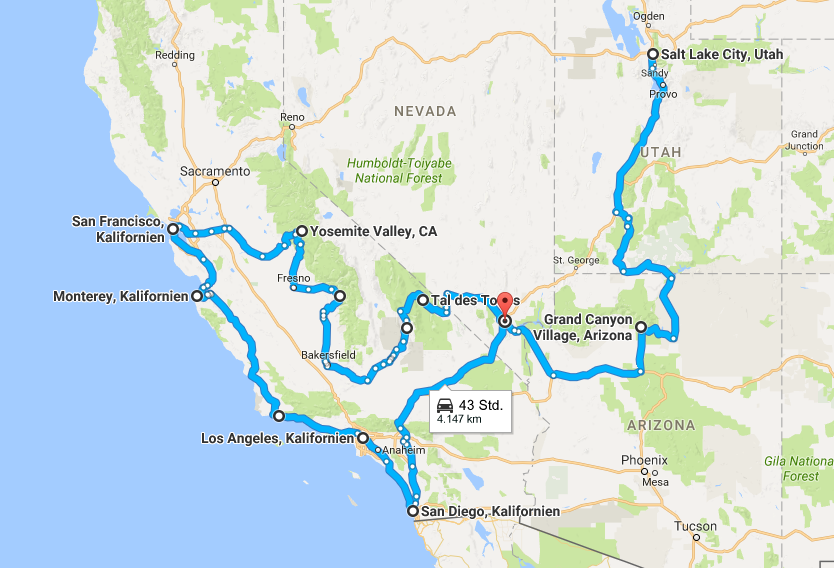
\includegraphics[angle=0,width=\paperwidth,height=.5\paperheight]{route_kleiner.png};%
};
\end{tikzpicture}
\newpage

\noindent
durch zwei zu teilen.
Wobei eine Übernachtung für eine Person nicht sonderlich günstiger ist als eine Übernachtung für zwei.

In den drei Wochen haben wir insgesamt 4646,43~€ durchgebracht. Dabei entfallen 1741,66~\$ auf die Übernachtungen, 1470,50~\$ auf Essen und Getränke und im Rest steckt der Benzin, der Mietwagen, die Einkäufe und die Tickets für die Attraktionen und National Parks.
